% !TeX spellcheck = en_US
%\documentclass[11pt,a4paper]{article}
\documentclass[11pt
  , a4paper
  , article
  , oneside
%  , twoside
%  , draft
]{memoir}

\usepackage{control}
\usepackage{kotex}
\usepackage[numbers]{natbib}
%\usepackage[pdftex]{graphicx}
%\DeclareGraphicsExtensions{.pdf,.png,.jpg}
\begin{document}

\newcommand{\technumber}{
  Low-Power Real-Time Scheduling\\
  Document 1: 2016-06-02}
\title{\textbf{Real-Time Dynamic Voltage Scaling for Low-Power \\
		Embedded Operating Systems \\
		요약 \\}}

\author{이상일\thanks{silee7103@ibs.re.kr} \\

  학번: 201460437\\
  Computer Engineering, Chungnam National University 
}
\date{\today}

\renewcommand{\maketitlehooka}{\begin{flushright}\textsf{\technumber}\end{flushright}}
%\renewcommand{\maketitlehookb}{\centering\textsf{\subtitle}}
%\renewcommand{\maketitlehookc}{C}
%\renewcommand{\maketitlehookd}{D}

\maketitle

\begin{abstract}
어플리케이션이 점점 정밀하게 됨에 따라서, 그리고 프로세싱 파워의 증가, 이러한 장치들에 대한 가장 심각한 제한은 사용 가능한 배터리 수명이다. 다이나믹 전압 스케일링 (DVS)는 공급 전압과 동작 주파수를 낮춤으로써 에너지 소비를 줄이기 위해 프로세서의 하드웨어 특성을 이용하는 것이 주요 기술이 되어왔다. DVS 알고리즘은 범용 시스템에서 필요한 최대 컴퓨터 사용 전력을 제공하는 동안에 극적 에너지 절약을 가능하게 해준다. 그러나, 휴대폰과 캠코더, 가변성 오퍼레이팅과 같은 임베디드 실시간 시스템에서 어플리케이션의 큰 클래스를 위해,  가변적으로 주파수를 운영하는 것은  그들의 데드라인 보증 메커니즘을 방해한다. 그것의 증가하는 중요성에도 불구하고, DVS는 주로지 간과 되거나 아직 개발 중에 있다. 실시간성을 보증하기 위해, DVS는 데드라인과 실시간 태스크의 주기성을 실시간 스케쥴러와 통합하여 고려하여야 한다.이 논문에서는 우리는 운영체제의 실시간 스케쥴러와 real-time deadline 보증을 유지하는 동안 중요한 에너지 절약을 제공하는 태스크 메니지먼트 서비스를 수정하는 “real-time DVS(RT-DVS) 라 불리우는 novel 알고리즘의 한 class를 제공한다. 우리는 이 RT-DVS  알고리즘이 밀접하게 에너지 소비에 대한 이론적 하한선에 접근한 것과 임베디드 실시간 시스템에서 에너지 소비를 20\%에서 40\%까지 쉽게 줄일 수 있다는 점을 시뮬레이션 및 프로토타입 구현을 통하여 살펴볼 것이다. 
\end{abstract}
\clearpage

\chapter{Introduction}
계산능력과 커뮤니케이션은 플랫폼 및 장치를 이동성 및 휴대가 가능한 방향으로 계속해서 성장시켜왔다. 이는 임베디드 시스템 분야에서도 발전해 왔으며, 계속되고 있는 소형화와 증가하는 컴퓨터 사용 전력으로, 우리는 디지털 캠코더, 휴대폰 그리고 휴대용 의료기기를 포함하여 장치의 방대한 분야에서 세련되고 지능적인 제어 소프트웨어를 실행하는 강력한 마이크로프로세서의 사용증가가 이루어짐을 보아왔다. 불행하게도 이런 장치(모바일 시스템)들의 뒤면에는 고유의 충돌이 있으며, 그러한 기기들의 배터리 수명을 극대화 하여야 하지만, 지능형 장비들은 더욱 많은 에너지를 소비하는 파워풀한 프로세서가 필요하다.더불어 배터리 수명도 저하된다.마이크로프로세서가 에너지 단위당 보다 큰 계산능력을 제공하고, 전체 배터리 수명을 증가시키는 반도체와 배터리 기술의 연속적인 발전에도 불구하고, 성능과 배터리 수명 사이의 기본적인 트레이드 오프는 중요한 사항으로 존재하고 있다. 현재 다이나믹 전압 스케일링(DVS)는 컴퓨터 시스템의 가장 중요한 특성인 두 가지를 고려함으로써, 성능과 배터리 수명 사이의 트레이드 오프를 다루려고 한다. 

\begin{itemize}
	\item 필요한 최대 컴퓨팅 비율이 유지하여야 하는 평균 처리량보다 훨씬 높다는 점
	\item 프로세서는 CMOS Logic으로 기본 되어야 함
\end{itemize}
 
첫번째 특성은 고성능은 시간의 작은 일부를 위해 단지 필요하며, 남은 시간을 위해서는   저성능, 저전력 프로세서로도 충분하다는 점이다. 우리는 full Speed 가 필요하지 않는 경우에, 프로세서의 동작주파수를 낮춤으로써, 간단하게 원하는 성능을 달성할 수 있다. DVS는 이것을 넘어서, 주파수와 함께 프로세스의 동작전압을 스케일링한다. 공급전압에 CMOS 회로소자 당 에너지가 분산되기 때문에 DVS는 잠재적으로 주파수와 전압 크기 조정을 통하여 매우 큰 에너지 절약을 제공할 수 있다. 시간이 제약된 어플리케이션에서, 휴대폰과 디지털 비디오 카메라와 같은 임베디드 시스템에서 종종 DVS 가 심각한 문제를 제공하는 것이 발견된다. 이러한 실시간 임베디드 시스템에서 알려진 대부분의 DVS 알고리즘을 직접 적용할 수는 없다. 왜나하면, 프로세서의 동작 주파수를 변경하는 것은 태스크의 실행 시간에 영향을 주고, 적시성 보장 일부에 대해 위반할 수 있기 때문이다. 이 논문에서는 우리는 실시간 임베디드 시스템의 OS 스케쥴러와 태스크 매니지먼트 서비스에 DVS를 통합하는 여러 새로운 알고리즘을 제공할 것이며, 데드라인을 보장하는 동안에 DVS의 에너지 절약을 제공할 것이다.이것은 현재의 DVS 알고리즘의 전형적인 평균 출력 기반 메커니즘과는 명백한 차이를 나타내고 있다.우리의 알고리즘의 에너지 보존 유용성을 보여주는 상세적인 시뮬레이션뿐만 아니라, 동작 시스템 측정을 통한 증명을 통해서 우리의 메커니즘의 실제적 구현(RT-DVS)을 보여주고 있다. 다음 장은 DVS의 세부사항, 실시간 스케쥴링, 그리고 우리의 새로운 RT-DVS 알고리즘을 나타낼 것이다. 3장에서는 시뮬레이션 결과 그리고 RT-DVS의 잠재적인 에너지 절약에 대부분의 영향을 미치는 시스템 파라미터에 대한 통찰을 제공할 것이다. 4장은 획득된 약간의 측정과 동작 시스템에서의 RT-DVS 메커니즘에 대한 우리의 구현을 설명할 것이다. 마지막 장에서 결론과 향후 방향에 대하여 우리의 업무를 논의할 것이다.   
 
\chapter{Real-Time DVS}
실시간 데드라인 보장을 요구하는 시스템에서의 에너지-절약 DVS 능력을 제공하기 위하여, 우리는 RT-DVS 알고리즘의 한 종류를 개발했다. 이번 장에서 일반적 DVS를 고려해 본 후 임베디스 실시간 시스템에서의 제한을 논의해 보며, 이 제한적 환경에서 개발한 RT-DVS 알고리즘을 나타낼 것이다.

\section{DVS}
전력 요구사항은 제한된 전력 소비, 짧아진 배터리 수명, 그리고 증가된 크기 및 무게로 디바이스를 제한하는 모바일 컴퓨팅 어플리케이션에서 가장 크리티컬한 제한 사항 중 하니이다.휴대용 또는 모바일 장치는 이러한 특성들 간의 트레이드오프를 고려하여 설계하여야 한다. 예를 들어 휴대용 컴퓨터 디바이스/플랫폼에 대한 고정된 사이즈와 무게가 주어졌을 때, 긴 배터리 수명을 제공하는 저속, 저전력 프로세서를 사용하여 시스템을 설계 할 수 있지만 성능이 저하된다.또는 모든 컴퓨팅 로드를 처리할 수 있는 파워풀한 프로세서를 탑재한 시스템 이지만 빈번한 배터리 재충전을 요구한다. 이런 이유로 본 논문에서의 논의사항은 2가지 주요 이유 로 휴대용 컴퓨팅 디바이스에서의 프로세서의 에너지 소비에 논점을 맞출 것이다.   
첫째로, 주어진 배터리 기술에 대해서 디바이스의 실제 크기 및 무게는 고정되어 있으며 이용가능한 에너지 역시 고정되어있다.둘째로, 우리는 특히 프로세서에 초점을 맞추었다.이유는 프로세서가 대부분의 시스템에서 가장 에너지를 많이 소비하는 소자이기 때문이다.문제에 대한 결론을 요약하면 프로세서의 Computing Power와 시스템의 배터리 수명은 트레이드 오프로 나타난다. 따라서 Computation을 성능이 만족하는 범위에서 특정 고비용 사이클 구간에 한정적으로 적용하여 에너지 소비를 줄인다. 이를 구현하는 하나의 메커니즘으로 DVS가 해당된다.DVS는 특별한 하드웨어에서 의존한다. 특히, 프로그래머블한 DCDC 스위칭 전압 레큘레이터, 프로그래머블한 clock 발생기, 그리고 넓은 동작 범위를 갖는 고성능 프로세서가 양쪽 계통(고성능 및 저전력) 의 최고의 능력을 제공한다. 최대 계산 로드를 충족시키기 위하여, 프로세서는 그것의 정상 전압와 주파수에서 동작한다.부하가 낮을 때, 동작 주파수는 계산 요구도를 충족하기 위하여 줄어든다.
DVS는 최대 계산 요구를 충족하기 위한 성능을 제공하며 평균적인 구간에서 
줄어든 전력소모(단위 계산당 에너지를 포함하는)를 제공하여 저성능의 프로세서상에서 동작하는 이점을 얻는다.      

\section{Real-time issues}
상위의 설명에도 불구하고, time-critical application에서는 주파수 스케일링은 문제가 될 수 있다. 특히, 휴대용 의료기기 및 핸드폰과 같은 실시간 임베디드 시스템에서, 태스크는 특정 데드라인 내에서 완료되어져야 하며, 지금까지 알려진 DVS를 위한 대부분의 알고리즘은 적용할 수 없다.이러한 DVS 알고리즘은 실시간 제약사항의 고려 없이 단순 평균 계산량에 근거하기 때문이다.일반적으로, 이 DVS 알고리즘은 단순한 피드백 메커니즘을 사용한다. 시간에 걸쳐 프로세스 상에서 대기 시간의 량을 감지함하고, 그런 후 주파수와 전압을 계산부하를 조정할 수 있게 조정한다. 이것은 매우 단순하며, 부하특성에 따른다. 하지만 어떠한 적시성도 보장하지 않으며, 태스크는 그들의 실행 데드라인을 놓칠 수 있다.일반적으로, DVS 알고리즘에 기초한 평균 처리량은 실시간 데드라인을 보장한다는 것은 어느 문헌에서도 찾을 수 없다. 실시간 임베디드 시스템에서 DVS의 줄어든 에너지 소모 이익을 실현하기 위하여, 우리는 동작 시스템상에서 실제 리얼타임 스케쥴러와 새롭게 간결한 DVS 알고리즘이 필요했다. 리얼타밍 시스템의 전통적인 모델에서, 주기적으로 실행되는 것이 필요한 태스크 세트가 존재한다. 

이 논문에서는 우리는 DVS 메커니즘을 2개의 가장 많이 연구된 실시간 스케쥴러 
RM 과 EDF 스케쥴러에 통합하기 위한 알고리즘을 개발하였다. RM 은 정적 우선순위 스케쥴러로, 태스크 우선순위를 주기에 할당한다.그것은 항상 짧은 주기를 갖는 태스크를 먼저 선택하는 것이다. EDF는 마감시간에 의해 태스크를 분류하는 동적 우선순위 스케쥴러로써 가장 마감시간에 가까운 태스크에 높은 우선 순위를 부여하는 것이다.
실시간 시스템에 대한 DVS에 대한 우리의 설계에서, 우리의 주요 목적은 에너지 소모를 줄이는 것이기 때문에,  우리는 일반적인 스케쥴링 메커니즘을 derive 하기 보다는 같은 가정을 유지하고 있다.  

\section{Static Voltage Scaling}
우리는 먼저 실시간 스케쥴링 능력을 유지하는 동안 전압 조절을 제공하기 위해서 단순한 메커니즘을 제안했다. 이 메커니즘에서, 우리는 주어진 태스크 셋을 위해 모든 마감시간을 충족할 수 있는 RM 또는 EDF 스케쥴러를 허용하는 가장 낮은 가능한 동작 주파수를 선택했다. 이 주파수는 정적으로 설정되었고, 태스크 셋이 변경되지 않는 한 주파수도 변경되지 않는다.적합한 주파수를 선택하기 위하여, 우리는 먼저 동작 주파수를 조절하는 것을 관찰했다.우리는 실시간 시스템 문헌들로부터 EDF와 RF 스케쥴러를 위한 잘 알려진 스케쥴링 테스트를 수행했다. 태스크의 필요한 최악의 계산 경우를 위하여 조절된 값들을 사용하였다. 특정 주파수에서의 스케쥴링을 위한 시험을 수행할 수 있다.이상적인 EDF 스케쥴링 아래에 있는 태스크 셋에 대한 필요하고 충분한 스케쥴빌리티 테스트는 최악의 경우 활용의 합계가 하나 이하일 것을 요구한다.스케일된 계산 시간값을 사용하여, 주파수 조정 factor를 가진 EDF 스케쥴러빌리티 테스트를 획득한다.유사하게 우리는 충분한 조건을 가지고 시작했다. RM 스케쥴링 하에 스케쥴링 는력을 위하여 
그리고, 조절된 주파수를 위한 테스트를 획득했다. 선택된 동작 주파수는 가장 낮은 주파수 중 하나로, 수정된 스케쥴러블 테스트는 성공했다. 물론 전압은 동작 주파수에 매칭하도록 변경된다. 동작주파수와 소프트웨어로 제공된 테이블 내에서 규정된 특정 하드웨어 플랫폼에 적용가능한 전압을 가정했다. 그림1은 EDF 와 RM 스케즐러에 대한 정적 전압 조절을 요약하고 있다.그림 2는 이 메커니즘을 나타내고 있고, 정적으로 조절된 EDF 와 RM 스케즐링하에서의 최악의 경우의 실행 기한을 나타내고 있다.이 예에서 테이블 2에서의 태스크는 각 테스크 기한 과 최악의 계산시간을 나타내고 있고, 3개의 nomalized, 독자적인 주파수 (0.5, 0.75, 1.0)이 가능함을 가정하였다.이 그림은 또한 EDF 와 RM 사이의 차이를 나타내고 있으며, 정적으로 조절된 RM이 EDF 버전처럼 적극적으로 주파수를 줄일 수 없음을 보여주고 있다. 일부 가능한 주파수에 한하여, 태스크 셋은 스케러블한 테스트를 통과하였고, 태스크가 그들의 조정된 계산 시간보다 더 사용되어지지 않는 한 이 단순한 메커니즘은 주파수와 전압조정이 그들의 데드라인까지의 태스크의 적절한 시행과 절충하지 않을 것이다.특별한 태스크 셋에 대하여 정적이고 태스크 셋 자체가 변경될 때만 선택된 주파수와 전압 설정은 바뀐다.결론적으로, 이 메커니즘은 실시간 운영체제 시스템의 태스크 매니지먼트 기능과 강하게 결합될 필요는 없고, 구현을 단순화하는 것이다. 다른 한편으로는, 이 알고리즘은 주파수와 전압조정을 통하여 전체적인 에너지 절감의 잠재력을 실현하지는 않을 것이다. 특히, 정적 전압크기 조정 알고리즘은  태스크가 프로세서 사이클의 최악의 경우 요구사항 보다도 이하로 사용되는 상황에 대해서는 다루지 않을 것이다. 이 공통적인 상황을 다룸에 있어서, 우리는 정교한 RT-DVS 메커니즘을 필요로 한다.           

\section{Cycle-conserving RT-DVS}
실시간 태스크가 최악의 계산요구도로 규정될 지라도, 그들은 일반적으로 대부분의 invocations 상에서 worst case 보다는 매우 적게 사용되어진다. 이것의 가장 좋은 이익을 취하기 위해서, DVS 메커니즘은 태스크가 그들의 worst-cast time allotment 보다 덜 사용되고, worst-case 요구를 충족하기 위해 주파수를 증가시킬 경우에, 동작주파수와 전압을 감소시킬 수 있다. 태스크가 그것의 다음 인보케이션을 위하여 배포될 때, 우리는 실제로 얼마나 많은 계산이 요구될지 알수가 없다, 그래서 우리는 그것이 규정된 최악의 경우의 프로세스 시간을 필요로 한다는 보수적인 가정을 반드시 하여야만 한다.태스크가 끝났을 때, 우리는 최악의 경우에 대한 규격을 사용하기 위한 실제 프로세서 사이클을 비교할 수 있다. 태스크에 할당된 어떤 미사용된 사이클도 정상적으로, 프로세서를 대기시키면서, 소모된다. 여분의 프로세스 사이클에 대한 대기하는 대신에, 우리는 동작주파수를 감소시킴으로써, 소모되는 사이클을 회피하기 위한 DVS 알고리즘을 고안할 수 있다. 
이것은 다소 슬랙 시간을 훔치는 것과 유사하다. 더 많은 일들을 달성하기 보다는 낮은 CPU 주파수에서 남아있는 다른 태스크들의 수행하기 위해 잉여시간이 사용되는 것을 제외하고는, 이러한 알고리즘은 운영체제의 태스크 매니지먼트 서비스로 강하게 결합되어 있다. 그들이 각각의 태스크 종결에서 주파수를 감소시킬 필요가 있고, 그리고 각각의 태스크 배포에서 주파수를 증가시킬 필요가 있기 때문에, 
그러한 알고리즘을 디자인하는 것에 있어서의 주요 도전은 동작주파수가 감소할 때 데드라인을 넘지않는다는 것 (보장)을 확실히 보장하는 것이다. 

test:
EDF 스케쥴링을 위해, 앞서 언급한바와 같이, 우리는 단순한 스케쥴러빌리티 (스케쥴링 능력) 테스트를 가지고 있다. worst-cast 태스크 활용의 합계가 더 결코 있지 않는 한, 태스크 셋은 factor에 의해 조정된 최대 주파수에서 동작될 때 스케쥴러블 하다. 만약 태스크가 그것의 최악수행시간 (worst-case computation time) 보다 빨리 끝난다면, 우리는 태스크에 의해 사용된 실제 계산시간을 사용함으로써, 우리는 재계산 활용에 의한 초과 시간을 교정할 수 있다. 
이 줄어든 값은 태스크가 다음 invocation 에 대해 다시 배포될때까지 사용된다. 
우리는 그림 3에서 이것을 묘사했다. 전과 같이 똑같은 태스크 집합과 가용 주파수를 사용하지만, 테이블 3에서 실제 실행시간을 사용함. 여기에서, 각 태스크의 invocation이 규정된 최악수행시간 보다는 사용되지 않는다. 하지만, 실제적인 값은 태스크가 실행을 완료한 후까지는 시스템에 알려질 수 없다. 
그러므로, 각 스케쥴링 포인트 (태스크 배포 또는 완료)에서, utilization은 완료된 태스크를 위한 실제 시간을 사용함으로써 재 계산된다. 그리고 다른 것들을 위한 규정된 최악의 경우와 주파수는 적절히 설정된다. 
그림의 수치는 각각의 포인트에서 이용 가능한 정보를 사용함으로써, 계산된 전체 태스크 활용을 보여준다. 알고리즘 자체는 단순하고 다음과 같이 수행된다. 
태스크 Ti 가 그것의 최악계산시간 Ci 보다는 일반적으로 작은 cci 사이클을 사용한 후 현재의 invocation을 완료했다고 가정하자. 태스크 Ti 가 그것의 현재 invocation에서 cci 사이클 보다는 더 사용되지 않기 때문에, 우리는 그것의 최악의 계산 범위(worst-case computation bound)가 cci 인 것처럼 태스크를 처리한다. 이 태스크를 위해 규정된 줄어든 utilization을 가지고, 우리는 태스크 셋이 스케쥴러블한 채로 남아 있는 것에 대해 지금 잠재적으로 더 작은 조정인자를 발견할 수 있다. 이 변화이전에 태스크 셋이 스케쥴러블 한 것이 주어진 경우 EDF 스케쥴빌리티 테스크는 계속 유지될 것이다. 그리고 Ti는 그것의 데드라인까지 시간이 남아있는 한 그것의 낮은 최대 계산 범위를 위반하지 않을 것이다.
그러므로, 태스크 셋은 적절히 실행을 보장하기 위해 실시간 스케쥴러에 의해 할당된 C1과 C2 조건을 모두 충족하기 위해 계속된다. 그리고 결과로써, EDF 스케쥴링에 의해 제공된 데드라인 보장은 Ti 가 다음 invocation을 위해 배포될 때 까지 최소한 적으로 계속하여 유지된다. 이 포인트에서, 우리는 Ci에 접근한 그것의 계산을 재저장하여야만 한다. 그것이 일시적으로 낮아진 경계를 위반하지 않을 것이며, 데드라인 보장을 절충한다는 것을 보장하기 위해- 이 시각에, 동작 주파수는 증가하는 것이 필요할지 모른다. 처음보면, 이 알고리즘은 현저하게 주파수, 전압, 그리고 에너지 비용을 감소시킨 것처럼 보이지 않는다. 그러나, 멀티 태스크가 줄어든 활용 단계에서 동시적으로 존재할 수 있기 때문에 전체적인 절약은 상당한 의미가 있다. RM 스케쥴링을 위한 cycle-conserving DVS 알고리즘을 설계하는 것은 같은 스케쥴러블리티 테스트 기반의 접근을 사용할 수 있다.하지만, RM 스케쥴러빌리티 테스트는 상당히 복잡하기 때문에, 우리는 여기 다른 접근을 취할 것이다. 우리는 태스크가 그들의 최악 실행시간을 항상 요구하고 있다고 가정하며, 이전에 논의된 정적 스케일된 RM 메커니즘이 실시간 데드라인 보장을 유지할 수 있다는 점을 주시하고 있다. 우리는 모든 태스크는 정적으로 스케일된 RM 알고리즘 하의 최악의 경우에서 보다는 여기서 만들어지고, 동작 주파수에 상관없이, 데드라인은 또한 여기에서 충족될 수 있다는 것에 대해 동일하거나 보다 좋은 과정이라고 주장하고 있다. 우리는 최악실행처리 패턴을 앞서기를 회피하려고 할 것이다. 이 것은 태스크에 의해서 사용된 실행 사이클에서의 어떤 감소도 동작주파수와 전압을 감소하는 방식으로 적용될 수 있다.이전의 같은 예제를 사용하여, 그림 5에서는 어떻게 이것이 이루어질 수 있는지를 설명한다.우리는 최초에 정적 스케일링에 기반한 최악의 스케쥴로 시작한다. (a) 이것은 예시에서 최대 CPU 주파수가 사용된다. 이것을 단순하게 유지하기 위하여, 우리는 시스템에서 다음 데드라인을 넘어서 보이지 않는다.우리는 그리고 나서 현재 시간으로부터 데드라인까지의 전체 interval을 걸쳐서, 이 데드라인 전에 작업이 완료되도록 하게 할 것이다. (b)이 것은 최소 동작 주파수 값을 제공한다. 하지만, 주파수가 discrete 하게 셋팅되고, 우리는 주파수를 1.0에 가깝게 셋팅하도록 할 것이다. 
T1이 실행된 후, 우리는 다음 데드라인(c)까지 남아있는 시간을 걸쳐서 남아있는 업무를 speading out을 수행하는 것을 반복한다. 그것은 그것의 최악으로 규정된 계산시간 보다 일찍 T1 이 완료되기 때문에, 더 낮은 동작 주파수에서의 결과가 된다.각각에 이것을 반복하면서 스케쥴링 포인트는 마지막 실행 trace 에서의 결과가 된다. 개념적으로 단순함에도 불구하고, 실제 알고리즘 (그림6)은 수많은 카운터가 반드시 유지되어야 하는 것 때문에 다소 복잡하다.이 알고리즘에서 우리는 각각 태스크 Ti를 위해,  계산의 최악의 경우 남아있는 사이클의 track을 유지할 필요가 있다.태스크 Ti 가 배포될 때, c lefti 가 Ci 로 설정된다.우리는 RM  메커니즘을 스케일링시키는 스태틱 전압이 시스템에서 임의의 태스크를 위한 가장 이른 데드라인에 의한 최악의 경우에서 만들어 지는 것을 결정한다.우리는 sj 와 sm, 그리고 다음 데드라인의 수를 획득했고, 정적-scaled에서의 동작과 최대 주파수를 가정하고 있다.sj 사이클은 RM 우선순위 order 에 따라서 태스크에 할당된다. 각 태스크 Ti 는 이 interval에 걸쳐서 정적 scaled 된 RM 시나리오 하에서 실행되는 사이클의 수에 따라서 allocation di c lefti을 수신한다. 
각 태스크 Ti 에 대해 다음 태스크 데드라인까지 di 사이클에서 실행되는 한, 우리는 최악의 시나리오에 보조를 맞추고 있다. 그래서, 우리는 d 값의 합을 사용하여 실행 속도를 설정한다.태스크가 실행됨에 따라서, 그들의 c 가 남고 d 값은 감소를 나타낸다.태스크 Ti가 완료될 때, c lefti and di는 0 값으로 설정되며, 주파수와 전압은 변경된다.우리는 동작 주파수를 선택하기 위해 이 기준을 사용한다. 이 알고리즘은 어떤 태스크 데드라인에서도 보장하며, 모든 태스크는 최악경우의 정적 스케일 RM 스케쥴에서 실행을 완료하여야 하며, 또한 그러므로 모든 마감에 맞추면서, 여기에서 모든 데드라인을 충족했을 것이다.
이 알고리즘은 다이나믹하게 주파수와 전압을 조정하면서, 실시간 태스크의 실제 계산 요구사항에 반응한다.기껏해야, 그들은 호출당 태스크에 2개의 주파수/전압 스위칭을 요구한다. 그래서 어떤 하드웨어 전압변경에 대한 임의의 오버헤드도 태스크들의 최악의 계산 시간 할당에서 설명될 수 있다.우리가 나중에 보일 것처럼, 알고리즘은 실시간 보증에 영향을 미치는 것 없이 중요한 에너지 절약을 달성할 수 있다. 

\section{Look-Ahead RT-DVS}
우리가 이 논문에서 소개한 최종 RT-DVS 알고리즘은 미래에 필요한 계산을 결정하고, 태스크 실행을 연기 하는 것을 결정하기 위해 look-ahead 기법을 사용하여 보다 좋은 에너지 절감을 달성하려 시도한다.사이클 보전 접근은 위에서 최초에 최악의 경우를 가정하였고, 일부 태스크가 완료될때까지 높은 주파수에서의 실행되는 것과 그리고 동주파수와 전압을 낮추는 것에 대해 논의했다. 대조적으로 look-ahead 구조는 가능한 많은 일을 유예하려고 시도하며, 미래의 모든 데드라인을 충족하는 것을 보장하기 위하여 지금 행하여질 최소한의 작업을 충족시키기 위해 동작 주파수를 설정한다. 물론, 이것은 제 시간에 연기된 모든 작업을 종료하기 위하여 나중에 고주파에서 동작하도록 강요받는다. 다른 한편으로는, 만약 태스크가 최악의 계산 시간 할당 이하로 사용되는 경향이 있다면, 연기된 작업을 위한 최대 실행 처리 비율이 결코 필요하지 않을지도 모른다. 그리고 이 휴리스틱은 그들의 데드라인까지 모든 태스크가 완료되는 동안에 시스템이 계속해서 낮은 주파수와 전압에서 동작하도록 허용할 것이다.이전의 사용된 예제에서 계속해서, 우리는 그림 7에서 lookahead RT-DVS EDF 알고리즘이 어떻게 동작되는지를 묘사한다.목적은 시스템(D1)에서 가장 이른 데드라인을 넘어서 작업을 연기하는 것이다 따라서, 우리는지금 낮은 주파수에서 동작할 수 있다.최근 데드라인, T3을 가진 태스크로 시작하면서, 우리는 각각 태스크의 최악의 경우 실행을 위한 스케줄에서 시간을 배정한다.우리는 D1과 그 자체의 데드라인 사이의 T3의 작업, 다른 태스크 (a)의 장래 호출을 위한 제약 비축 용량에 따른 D3을 펼쳐졌다. 우리는 T2를 위한 이 단계를 반복하며, 그것은 T1의 장래 호출을 위해 T3과 비축 용량을 배정한 후에, 전적으로 D1과 D2 사이를 적합할 수는 없다. T2를 위한 추가적인 작업과 모든 T1의 모든 것은 D1이전에 할당된다.우리는 D2이후에 T3의 모든 것을 이동했더라면, T2의 더 많은 것들이 D1을 넘어서 유예될 수 있다는 점을 주목했다. 하지만 단순히 이것은 고려되지 않는다.우리는 동작 주파수를 결정하기 위해 D1 앞에 배정된 일을 사용한다.규정된 최악의 실행 사이클 보다 낮게 사용되어, 한번 T1이 완료되면, 우리는 이것을 반복하고, 더 낮은 동작 주파수를 찾게 된다.궁극적으로 시스템에서 다음 데드라인을 넘어서는 작업을 유예하기 위한 시도는 계속되며 (f) 에서 실행 흔적에서 결과가 나타난다.EDF 스케쥴링을 가진 look-ahead RT-DVS를 위한 실제 알고리즘은 그림 8에서 제시된다. RM을 위한 사이클-보전 RT-DVS 알고리즘에서와 같이, 우리는 태스크 Ti의 현재 호출을 위하여 최악의 경우 남겨진 계산 c lefti 의 track을 유지한다. 이것은 태스크 배포에서 Ci로 셋팅되며, 태스크가 실행된 것처럼 감소하고, 그리고 종료 상에서 0으로 설정된다. 이 알고리즘에서 주요 단계는 deferral 기능이다. 여기에서, 우리는 다음 태스크 데드라인까지의 간격을 보고, 데드라인까지 넘어서 할 수 있는 것처럼 많은 작업을 수행하려 하고, 그리고 s 사이클의 최소 수를 계산하고, 모든 미래 데드라인을 충족하기 위하여 이 간격 동안 실행하여야 한다.동작 주파수는 이 간격을 거쳐서 s 사이클을 실행하기 위해 충분히 빠르도록 설정된다.계산을 위해, 우리는 reverse EDF 순서에서 태스크를 주시한다.이른 데드라인을 가진 태스크에 의한 최악의 경우 활용을 가정하므로써, 우리는 사이클 x의 최소 수를 계산할 수 있다. 태스크는 반드시 가까운 데드라인 Dn  이전에 실행되어야 하며, 그것 자신의 데드라인에 의하여 완료되어야 한다.누적된 활용 U는 Dn 뒤에 시간 동안 태스크의 실제 사용을 반영하기 위해 조절된다. 이 연산 s는 태스크에 대한 반복이며, 이른 데드라인 태스크를 위한 예측된 최악의 경우 활용 값과  나중의 데드라인를 위한 계산된 값들을 사용한다. s는 간단하게 태스크에 관한 한 계산된 x 값의 합계이고, 그러므로 그들의 데드라인을 충족하기 위하여  모든 태스크를 위한 Dn에 의해 실행할 사이클의 전체 수를 반영한다. 이 알고리즘이 매우 적극적으로 프로세서 주파수와 전압을 감소시킬지라도, 상위 우선 순위 (더 초기 데드라인) 태스크에 대비하여 최악의 경우 요구사항을 남겨 둔 후 그것의 데드라인에 맞추는 것이 각각 태스크에 이용 가능한 충분한 사이클이 있다는 것을 그것은 확실하게 한다. 

\clearpage
\chapter{Simulations}
우리는 real-time scheduled system에서 voltage scaling으로부터 잠재적 에너지 절감에 대한 평가를 하기 위한 simulator를 개발하였다. 다음 서브 섹션은 simulator 설계에서 이루어진 가정 및 그것에 대하여 기술한다.
\section{Simulation 방법론}
우리는 C++를 사용하여 real-time scheduling상에서 전압과 주파수의 범위의 하드웨어 기능 동작에 대한 simulator를 개발하였다. Simulator는 여러 시스템 파리미터들 뿐만 아니라 각 task의 계산 및 period 요구사항을 갖는 “task set”을 입력받아, 우리가 개발한 알고리즘 각각에 대한 시스템 에너지 소비를 제공한다. 어떤 DVS 지원없이 EDM and RM 스케쥴러는 또한 비교를 위해 모사된다. Simulator에 제공되는 파라미터들은 machine 사양 (모사된 platform상에서 이용 가능한 votages 및 주파수의 lsit) 및 각 호출에 요구되는 최악의 실행 사이클의 실제 조각(actual fraction)에 대한 사양을 포함한다. 마지막 파라미터는 상수 (예를들어, 0.9는 각 태스크가 각 호출동안에 명시된 최악의 계산 사이클의 90\%를 사용한다는 것을 가르킨다. ) 또는 무작위 함수 (random function) (예를 들어 각 호출에 대한 균등분할 random multiplier). 시뮬레이션은 일정량의 에너지가 주어진 전압에서 동작의 각 싸이클 동안 요구되는 것을 가정한다. 이 양자는 CMOS 회로에서 에너지 소모와 일치하는 동작전압의 제곱에 비례한다. 프로세서에 의한 소비된 에너지 만이 계산되며, 실행된 서로 다른 타입의 instruction에 의한 변동은 계산되지 않는다. 이런 단순화로 태스크 실행 모델링은 실행 사이클을 카운팅을 줄이며, 실행 추적은 필요하지 않다. 소프트웨어 제어 폴트 특징(일부 프로세서에서 유휴기간동안 에너지 소비를 감소시키기위하여)은 idle level parameter를 명시하므로 모사된다. 이 값은 정지된 동안의 사이클 기간 중 소비된 에너지와 정상운전 사이클 기간 중의 소비된 에너지 사이의 비율의 값이다. (0.5 값은 계산 사이클 에너지의 1/2을 ideling 소비로 쓰여진 1 사이클을 가르킨다.) 간결성을 위하여, 태스크 실행과 idle 사이클 만이 고려된다. 특히, 선점과 태스크 절체의 오버헤드 또는 동작 주파수 또는 전압을 절체하기 위해 요구되는 시간은 고려되지 않는다. 이러한 단순성에 대한 일반성의 손실은 없다. 선점과 태스크 절체 오버헤드는 DVS가 있건 없건 동일하다. 그래서 상대적인 전력소비에 영향을 미치지 않는다.
전압 스위칭 오버헤드는 어떤 태스크 셋에 대한 스케쥴성에 영향을 줄 수도 있는 시간 페널티를 부과하지만. 프로세서는 스위칭 interval동안 동작하지 않으므로써, 거의 에너지 비용은 없다. 실시간 태스크 셋은 각 태스크에 대한 그것의 기간과 최악의 소비시간을 가르키는 숫자쌍을 사용하여 명시된다. 태스크 셋은 다음처럼 랜덤하게 생성된다. 각 태스크는 짧게(1-10ms), 중간으로(10-100ms), 길게(100-1000ms)를 갖는 동일한 확률을 갖는다. 각 범위안에, 태스크 기간은 동일하게 분산된다. 이것은 실시간 시스템에서 흔히 발견되는 짧고 긴 태스크 기간의 다양한 혼합으로 모사된다. 태스크의 계산 요구사항들은 유사한 3 범위 동일 분포를 사용하여 랜덤하게 할당된다. 결국, 태스크 계산 요구사항들은 태스크 셋안에 태스크들의 이용률의 합이 원하는 값에 도달하기 위한 선택 상수에 의한 범위를 갖는다. 이러한 실시간 태스크 셋을 생성하는 방법은 마이크로 커널을 임베디드한 실시간 평가로 이전부터 개발되어왔다. 여러 서로 다른 총 최악의 이용률 값에 대하여 생성된 수많은 고유 태스크 셋들의 평균을 취하여, 시뮬레이션은 태스크 셋의 최악의 이용률에 대한 에너지 소비의 관계를 제공한다.
\section{Simulation 결과}
우리는 에너지 소비에 영향을 미치는 가장 중요하고 관심이 있는 시스템 파라미터를 결정하기 위해 RT-DVS 알고리즘의 광범위한 시뮬레이션을 수행 하였다. 별도의 규정이 없는한, 우리는 3개의 상대 동작 주파수(0.5,0.75,와 1.0)와 그에 대한 전압(3, 4, 5) 를 제공하는 DVD-capable 플랫폼을 가정한다. 다음에 오는 시뮬레이션에서 우리는 각각 non-DVS 시스템과 우리의 RT-DVS 알고리즘을 비교한다. 우리는 또한 에너지 소비에 대한 이론적 하한 경계를 포함한다. 이 하한은 실행 처리량을 반영하고 어떤 타이밍 문제를 고려하지 않는다. 시뮬레이션에서 계산 작업 사이클의 총 수를 고려하여 계산되며, 주어진 플랫폼 주파수 및 전압 사양 시뮬레이션 시간 지속 기간동안 수행 될 수 있는 절대적인 최소 에너지를 결정한다. 실제 알고리즘은이 이론 하한보다 더 할 수 없다, 그러나 우리의 메커니즘이 결합 된 접근 얼마나 가까이 있는지 흥미로운 일이다.
태스크 수:
시뮬레이션 첫 세트에서 우리는 작업 세트 태스크의 수를 변화시키는 효과를 결정한다. 그림 9는 
수정되지 않은 EDF 뿐만 아니라 우리의 RT-DVS 알고리즘 모두에 대하여 5, 10, 15 태스크를 갖는 태스크 셋에 대하여 에너지 소비를 보여준다. 이러한 모든 시뮬레이션들은 모든 프로세서가 완전한 소프트웨어 제어 정지 기능을 제공한다고 가정한다. 추가로 우리는 태스크 각각의 호출 동안 최악의 경우의 연산 요구를 소비 할 것으로 가정한다. 극단적으로, 정적 스케일링주기와 보전 EDF 알고리즘 차이가 없다. 우리는 RT-DVS 알고리즘이 큰 에너지 절감 가능성을 보임을 즉시 확인하며, 미드 레인지 최악의 프로세서 사용률 값을 갖는 태스크 셋에 대하여 특히 인식한다. 이전 RT-DVS 메커니즘은 특히 이론 하한 경계에 매우 밀접하게 따르는 것으로 볼 수 있다. 총 사용량율이 크게 에너지 소비에 영향을 주더라도, 태스크의 수에는 거의 영향이 없다. 작업의 수가 변화되는 경우에 서로 다른 알고리즘에 대해 곡선의 절대 위치 또는 상태적 위치는 크게 이동하지 않는다. 태스크 수의 변화는 거의 효과가 없기 때문에, 더 많은 시뮬레이션에서 우리는 하나의 값을 사용한다.

지연 레벨 변화:
이전 시뮬레이션 완전한 소프트웨어 제어 정지 기능이 프로세서에 의해 제공되는 것으로 가정하였다. 그래서 유휴시간은 에너지를 소비하지 않는다. 불완전한 정지 기능은 전력 소비에 어떻게 영향을 미치는지 확인하기 위해, 우리는 유휴 레벨 인자를, 이는 프로세서가 정지되는 동안에 대하여 한 사이클에서 소비되는 에너지의 비율, 다양하게 하는 여러 시뮬레이션을 수행하였다. 정상적인 실행 사이클에서 소비되는 에너지, 그림 10은 지연 레벨 factor가 0.01, 0.1, 1.0에 대한 결과를 나타낸다. 소비 절대 에너지는 분명히 아이들 상태의 에너지 소비가 증가함에 따라 증가하기 때문에, 이는 수정되진 않은 EDF 에너지 소비에 대한 정규화된 값을 플로팅하여 상대적으로 에너지 소비를 보면 더욱더 확인 할 수 있다. 가장 중요한 결과는 non-energy 보존 스케쥴러가 가장 간결한 상태에서 보여지는 심지어 완전한 정지 기능은 아직도 RT-DVS 알고리즘으로 매우 큰 폭의 비율로 개선의 여지가 있다. 명백히 idle level을 1로 증가하여 전압 스케일을 가지고도 그 비율이 상승한다. 에너지 인식 스케줄러 간의 상대적 성능은 비록 동적 알고리즘이 정적 스케일링 것보다 더 많은 장점이 있더라도 크게 유휴 전력 소비 레벨을 변경함으로써 영향을 받지 않는다.
이는 사이클 보존 EDF 메커니즘이 정적 범위를 갖는 EDF 결과로부터 발산한다는 명백한 결과이다. 이는 동적 알고리즘이 idle 기간 중에 가장 낮은 주파수와 전압으로 전환된다는 사실을 쉽게 설명한다. 반면에 정적 알고리즘의 것은 그러하지 않다. 완벽한 idle의 경우 이것은 차이가 없지만, 
유휴 사이클 에너지 소비가 실행 사이클의 것에 근접할 때 동적 알고리즘은 상대적으로 좋은 성능을 낸다. 시뮬레이션의 나머지에 대해서는 우리는 유휴레벨을 0으로 가정한다. 

Machin 사양의 변경:
이전 모든 시뮬레이션은 가능한 주파수 및 전압 스케일링 설정의 한 세트 만을 사용 하였다. 우리는 이제 모사된 machine의 사양을 변경하면서 얻는 효과를 조사한다. 다음은 하드웨어 전압과 주파수 설정을 요약한다. 각 튜플은 상대적 주파수와 그에 따른 프로세서 전압으로 구성된다.
machine 0: f (0.5, 3), (0.75, 4), (1.0, 5) g
machine 1: f (0.5, 3), (0.75, 4), (0.83, 4.5), (1.0, 5) g
machine 2: f (0.36, 1.4), (0.55, 1.5), (0.64, 1.6),
(0.73, 1.7), (0.82, 1.8), (0.91, 1.9), (1.0, 2.0) g 

그림 11은 이전 모든 시뮬레이션에서 사용된 machine 0,1,2에 대한 결과를 보여준다. 이는 표준 PC 메인보드상에서 예상될 수 있는 주파수 설정값을 갖는다. 비록 해당 전압 레벨이 임의로 선정되었지만,
Machine 1은 추가 주파수 설정 0.83을 갖는다는 것에서 이것과 다르다. 이 작은 변경으로 우리는 이러한 사양에 대한 시뮬레이션 결과에 약간의 차이를 기대한다. 가장 의미있는 변경은 사이클 보존 EDF에서 보여진다. (정적 범위 EDF와 그 둘은 여기서 동일하다.) CCF와 ccRM 사이의 크로스 오버 포인트 근처 지역에서 별도의 동작점으로, ccEDF 알고리즘은 전 사용률에 크로스 오버점이 더욱 밀접해지는 shifting 이익을 얻는다. 
Machine 2는 나머지 두개와 매우 다르며 AMD의 PowerNow 메커니즘을 갖는 AMD K6 프로세서를 포함하는 플랫폼을 사용 할 수 있다는 설정을 반영한다. 다시 전압레벨은 여기에서 추측된다.
선택 가능한 더 많은 설정으로 그려진 곡선은 더욱 부드러워지는 경향이 있다. 
또한, 상대 전압 범위는 본 명세로 좀더 작기 때문에 최대 saving은 다른 두 machine의 명세만큼 좋지는 않다. 더욱 중요한 것은 사이클 보존 EDF가 look-ahead(예견) EDF 알고리즘보다 성능이 좋다는 사실이다. ccEDF 및 정적 EDF는 많은 설정에 대해 이익을 얻는다. 이것은 그 두 알고리즘에게 태스크 셋이 더욱 밀접하게 일치되어 에너지 소비를 줄일 수 있기 때문이다. 사실 그들은 매우 전체 범위를 넘어선 이론적 하한에 근사화 된다. 다른 한편으로  laEDF는 processing을 지연도록 하는 주파수를 설정한다.(최악의 경우 나중에 full speed에 실행을 요구하는) .
더 많은 설정으로 낮은 주파수 설정은 고전압 요구, 고주파 후처리, 성능 감쇠등에 밀접하게 일치된다. 더 적은 설정으로 설정된 주파수 좀더 높게되어 적은 processing이 지연된다. 이후 높은 전압과 주파수의 설정을 필요로 할 가능성을 줄이므로 성능을 개선한다. 어떤의미에서 주파수의 제한된 수로 인한 에러가 ccEDF 방식에 해가 되지만, laEDF로는 이익이 된다. 이러한 결과는, 따라서, 다양한 RT-DVS 알고리즘에서의 에너지 절감은 이용가능한 플랫폼의 전압 및 주파수의 설정에 크게 의존하는 것을 나타낸다. 
계산 시간 변경:
이런 일련의 실험에서 우리는 잘된 RT-DVS 메커니즘이 최악의 계산 시간을 소비하지 않는 태스크 셋에 어떻게 유리한지를 보여주기 위하여 각 호출 동안에 태스크에 의해 요구되는 실제 계산 의 분포에 변화를 가한다. 앞선 시뮬레이션에서, 우리의 작업이 항상 최악의 계산할당을 요구한다고 가정하였다. 그림 12는 각 호출에 대한 최악의 실행사이클의 일정한 90, 70, 50\%를 요구하는 태스크에 대한 시뮬레이션 결과를 보여준다. 우리는 정적으로 범위되어진 메커니즘이 영향을 받지 않음을 관찰한다. 왜냐면 그들이 태스크들에 명시된 최악의 계산 시간상에서 유일하게 근거한 전압과 주파수를 스케일하기 때문이다. 사이클 보존 RM 알고리즘에 대한 결과는 의미있는 변화를 보여주지 않는다. 그것은 그들의 지정된 최악의 경우 계산 시간 미만을 사용하는 작업에 적용이 매우 좋지는 않다는 것을 나타낸다. 다른 한편으로 두 사이클 보존 방식과 look-ahead EDF 방식은 실제 계산이 감소 수행되므로써 상대적인 에너지 소비에 큰 감소를 보여준다. 그림 13은 0과 최악의 계산 사이에서 단일 분산을 갖는 태스크들을 사용하여 시뮬레이션 결과를 보여준다. 소개된 랜덤에도 불구하고, 결과는 작업의 각 호출에 대해 지정된 값 절반에 대한 계산 설정과 동일하게 나타납니다. 이는 단일 분배를 갖는 평균 실행이 각 태스크에 대하여 최악의 0.5배가 됨을 의미한다. 이것으로부터, 호출당 연산의 실제 분포는 에너지 절약 성능에 중요한 요인이 아니라고 보인다. 대신 동적 메커니즘 들면, 상대적인 에너지 소비량을 결정하는것은 평균 사용률이다. 반면 정적 스케일링 방법은 최악 사용율이 결정적인 요소이다. 예외는 태스크 셋의 최악의 사용율을 주로 반영하는 결과를 갖는 ccRM 알고리즘이다.

\chapter{Implementaions}
이 절에서는 제안 된 DVS 알고리즘을 포함하는 실시간 예약 시스템의 우리의 구현에 대해 설명한다. 우리는 시스템 구조 및 우리의 RT-DVS 알고리즘으로 실제 에너지 절약의 현재 측정을 설명한다.
\section{Hardware Platform}
우리는 주로 실시간 임베디드 장치에 대한 RT-DVS 메커니즘을 개발했지만, 우리 프로토타입 시스템은 PC 아키텍처로 구현된다.플랫폼은 550 MHz의 최대 동작 주파수를 갖는 AMD K6-2 + [1] 프로세서가 휴렛팩커드 N3350 노트북 컴퓨터이다. 이 노트북에서 측정 된 소비 전력 숫자들 중 일부는 이전에 표 1에 나타내었다. 이 프로세서의 특징들은, PowerNow, 소프트웨어 제어로 프로세서의 클럭 주파수 와 전압을 조정될 수 있는 AMD의 확장이다. 우리는 또한 speedStep으로 불리는 intel에서 유사한 것을 보았지만, 이것은 프로세서 외부 하드웨어를 통해 전압 및 주파수를 제어한다. 비록 소프트웨어 제어로 설정을 가능 할 지라도, 우리는 외부 하드웨어를 제어하기 위해 필요한 적절한 출력 시퀀스들을 결정할 수 없었다. 우리는  Transmeta Crusoe 프로세서 또는 DVS를 지원하는 다양한 임베디드 프로세서에 대한 경험이 없다. The K6-2+ 프로세서 사양은 시스템 소프트웨어가 내장된 PLL 클럭 발생기로부터 8개의 서로 다른 주파수들 중 하나를 선택할 수 있도록 한다(200 ~ 600 MHz in 50MHz 증가분, 250 제외). 프로세서는 외부 조절기를 통해 전압을 설정하는 데 사용할 수 있는 5개의 제어 핀을 갖는다. 32개의 설정이 가능하지만, 명시적으로 하나가 지정된다(the default 2.0V setting); 나머지는 개별 제조사에 달렸다. HP는 유일하게 2개의 전압 설정하도록 선택하였다.(1.4v, 2.0v) 전압 및 주파수 선택기는 독립적으로 설정할 수 있으므로 적절히 가능한 전압 레벨로 각각의 주파수에 매핑하는 기능을 해야한다. 공개적으로 사용가능한 명세서들이 없기에 우리는 이것을 실험적으로 결정하였다. 프로세서는 1.4v에서 450MHz까지 안정하며, 좀 더 높은 주파수에 대해서 2.0v 설정이 필요한다. 안정상은 CPU-intensive benchmark의 셋을 사용하여 검증하였다. 우리는이 경험적인 연구는 하나의 샘플 크기를 사용주의, 그래서 전압 매핑 실제 주파수는 심지어 같은 모델의 다른 컴퓨터에 따라 다를 수 있습니다. 우리는 이 경험적인 연구가 하나의 샘플 크기를 사용하고 그래서 주파수 맵핑에 대한 실제 주파수는 다른 machine에 따라 다양하며 심지어 같은 모델에 대해서도. 프로세서는 주파수 전이 또는 전압의 매변화에 대한 프로세서 실행을 멈주게 하는 동안 연계된 강제 정지 구간을 갖는다. 강제적 정지 구간은 전압 공급 및 클럭 프로세서가 실행을 계속하기 전에 안정화 시간을 가질 수 있도록하는 것을 의미한다. 크게 달라질 수 외부 전압 조절기의 상이한 하드웨어 구현의 특성으로, 이 정지 기간은 41us (4096 cycles of the 100 MHz system bus clock)의 배수로 프로그램가능하다. 경험에 따라, 주파수의 변화가 발생하는데는 무시할 만한 시간이 걸린다. 정지기간동안에 계속 count하는 CPU 타임 스탬프 레지스터를 사용하여, 우리는 약 8200 사이클이 200MHz, 그리고 약 22500 사이클이 550MHz에 전환하는 것을 관찰한다. 둘은 41마이크로 세컨드의 최소 인터벌을 가지고. 이것은 CPU 클럭의 주파수가 신속히 변화하고 정지 시간의 대부분이 목적 주파수에 소요되는 것을 가리킨다. 우리는 전압 전환이 발생하는 데 필요한 실제 시간을 모르지만, 우리의 실험에서 10의 정지 기간 값을 사용하여 불안정성이 관측되지 않는 결과를 냈다. 따라서, 스위칭 오버 헤드가 우리의 시스템에 전압이 변경 될때 0.4ms 이고, 주파수만이 변할때는 41 us이다. 앞서 언급되었듯이, 최대 두 개의 전환이 각 호출에서 각 작업에 기인하기 때문에 우리는 작업의 계산 요구 사항에서 스위칭 오버 헤드를 고려 할 수 있다.

\section{Software Architeture}
우리는 리눅스 커널 2.2.16에 확장 모듈로 알고리즘을 구현했다. 비로 실시간 운영체제가 아닐지라도, 리눅스는 쉽게 모듈로 확장 되며 우리에게 익숙한 개발환경을 제공한다. 우리의 소프트웨어 아키택쳐의 상위 수준은 그림 14에서 보여준다. 이러한 구현에 수행된 방법은 성능을 최적화하는 것에 좀더 사용의 유연성 및 편리성을 극대화 하는 것이었다. 이 구현은 이상적인 모델이라기 보다는 다소 좋은 개념 증명으로 제공한다. 리눅스 커널 모듈로서 우리의 커널 레벨 코드를 구현하므로써, 리눅스 커널 어떤 코드 변경도 하지 않았다. 또한 이런 모듈들은 수정되지 않은 2.2.x kernels에 끼워 맞추어 질 수 있다. 우리 구현에 핵심 모듈은 리눅스에서 주기적 실시간 태스크에 대한 지원을 제공한다. 이것은 리눅스 스케줄러와 타이머 틱 핸들러 내부를 후크 콜백 함수를 부착하여 수행된다. 이 메커니즘은 우리의 모듈이 타이트한 타이밍 제어를 제공 할뿐만 아니라 기본 유닉스 스케줄링 정책을 우리의 실시간 작업에 대하여 대체 할 수 있습니다. 이 모듈은 실제로 실시간 스케줄링 정책 또는 DVS 알고리즘을 정의하지 않는다는 점에 유의한다. 대신 우리는 실시간 스케쥴링 정책 및 RT-DVS 알고리즘을 제공하는 모듈로 분리한다. RT 스케쥴러 / DVS 모듈이 하나로 한번에 시스템상에 적재될 수 있다. 주기적 RT 지원은 스케쥴링 정책 과 DVS 정책으정부터 분리하므로써, 이 아키텍처는 시스템 또는 실행중인 RT 작업을 종료하지 않고 후자의 정책을 동적으로 전환 할 수 있다. 이 아키텍처는 시스템 또는 실행중인 RT 작업을 종료하지 않고 후자의 정책을 동적으로 전환 할 수 있다. 본 구현의 마지막 커널 모듈은 PowerNow 메커니즘에 클럭 속도와 전압을 조정하기위하여 다룬다. 이는 어떤 요구되는 주파수 및 전압 레벨에 대한 프로세서의 특별한 특징 register의 적당한 bit 설정을 위한 상위수준 interface를 제공한다. 모듈은 리눅스 /procfs 파일 시스템을 통한 사용자 레벨 프로그램에 인터페이스를 제공한다. 태스크는 우리의 모듈과 상호작용하기 위하여 보통의 파일 read and write 메커니즘을 사용할 수 있다. 특히 태스크는 그것이 요구되는 기간 및 우리의 모듈에 최대 computing bound을 쓸 수 있다. 그리고 그것은 주기적으로 release 되고, 현재 로드된 정책 모듈에 따라 스케쥴되는 주기적 실시간 태스크로 만들어질 것이다. 그리서 시스템 상에서 비 RT 태스크를 넘는 정적 우선순위를 받게 될 것이다. 또한 사용하는 작업이 다음 릴리스 때까지 차단되는 시간에 각 호출의 완료를 나타내는 기록합니다. 또한 사용하는 작업이 다음 릴리스 때까지 차단되는 시간에 각 호출의 완료를 나타내는 기록을 사용한다. 태스크가 파일 핸들 open을 유지하는 동안, 그 태스크는 우리의 커널 확장을 갖는 실시간 태스크로 기록될 것이다. 비록 이 상위수준, 파일 시스템 interface가 직접 시스템 콜 만큼 효율적이지 못해도, 그것은 프로타입 구현에 편리하다. 왜냐면 단순히 우리는 cat을 사용하여 우리의 모듈로부터 읽을 수 있고 인간이 읽을 수 있는 형태로 상태 정보를 얻을 수 있다. PowerNow 모듈은 또한 /procfs interface를 제공한다. 이는 다른 DVS문헌에서 발견되는 알고리즘을 구현하는 사용자 레벨을 가능하게 하여 수동으로 간단한 유닉스 쉘 명령을 통해 동작 주파수와 전압을 처리한다.

\section{측정 및 관측}
우리는 RT-DVS구현을 가지고 여러 실험을 수행하였고 시스템의 실제 에너지 소비를 측정하였다. 그림 15는 에너지 소비를 측정하는데 사용된 구성을 보여준다. 노트북 배터리는 제거 되었고 시스템의 외부 DC 전원을 사용하여 구동한다. 별한 전류 프로브를 사용하여, 디지털 오실로스코프는 공급되는 전류와 전압의 곱으로 랩탑에 의해 소비되는 전력을 측정하기 위해 사용된다.
이 기본적인 방법은 PowerScope에서 사용 된 것과 매우 유사하다. 그러나 속도가 느린 디지털 멀티미터 대신 우리는 과도 동작을 확인할 수 있고 오랜 기간동안 실제 평균소비전력을 제공할 수 있는 오실로스코프를 사용한다. 디지털 오실로스코프의 장기간 획득 기능을 사용하여, 우리의 전력 측정은 15 ~ 30 초 간격에 걸쳐 평균화된다. 그림 16는 각 호출에 할당된 최악의 계산의 90\%를 항상 소비하는 5개의 태스크 셋을 위하여 최악의 CPU 사용률을 변화시키는 동안 우리의 RT-DVS 알고리즘을 위하여 측정된 실제 전력 소비를 보여준다. 측정은 전체 시스템 전력뿐 아니라 CPU 에너지 손실을 반영한다. 결과적으로 시스템 보드의 소비로부터 줄일 수 없는 상수의 파워 배출이 있다. (display backlighting은 이 측정을 위해 off 되었다; on 되었을시 추가적 상수 값 6w 측정된다). 이 오버헤드에도 심지어 우리의 RT-DVS 메커니즘은 전력소모에서 여전히 실시간 시스템의 데드라인을 만족하면서 의미로운 20~40\% 감소를 보여준다, 그림 17은 이 측정에서 동일한 매개변수로 시뮬레이션을 보여준다. (2개의 전압레벨 machine 사양을 포함하여). 시뮬레이션은 단지 프로세서의 에너지 소비를 반영하며 시스템의 나머지 부분에서는 어떤 에너지 오버헤드도 포함하지 않는다. 실제측정에서 일정한 오버 헤드의 추가를 제외하고, 결과들은 거의 동일하다. 시뮬레이터에서 단순한 가정들에도 불구하고, 이것은 우리가 이전에 보았던 결과들이 실제 시스템에서 실제로 유지되는 것을 보여주므로 우리의 시뮬레이션 결과가 유효함을 검증한다. 시뮬레이션들은 RT-DVS 구현의 성능을 예견하는데 정확하며 유용할 수 있다. 우리는 또한 RT-DVS를 갖는 시스템을 구현할 때 고려되어야 하는 두가지 현상에 주목한다. 첫째로 우리는 태스크의 바로 첫 호출이 그것의 명시된 계산 시간 경계를 오버런 할 수 있음을 주목한다. 이것을 첫 호출상에서만 발생하며 운영체제 상태와 “cold” 프로세서에 의해 원인이된다. 특히 태스크가 실행을 시작할 때 많은 캐시 misses, TLB misses 와 page fault가 시스템에서 발생한다(마지막은 리눅스에서 사용하는 기록 중 복사 페이지 할당 메커니즘에 기인 할 수 있다). 이러한 processing 오버헤드들은 태스크 실행 시간에 대하여 카운트하며, 그 경계를 초과하는 원인이 된다. 뒤에 오는 호출들상에서 그 상태는 “warm”이며, 이 문제는 사라지게 된다. 이는 일반적인 목적의 플랫폼상에서 최악의 경우와 평균의 경우의 성능 사이에 큰 차이를 내게 하며, 실시간 시스템이 성능의 이러한 변동을 제거하거나 줄이기 위해 특수 플랫폼을 사용하는 경향을 설명한다. 두번째 중요한 관측은 태스크 셋에 대한 태스크의 동적 추가는 한 태스크에 매우 주의를 하지 않는다면 과도한 미스된 deadline들에 원인이 된다. 특히 더욱 공격적인 RT-DVS 방식으로, 시스템은 새로운 태스크를 다루는데 태스크 데드라인 전에 남아 있는 프로세서 사이클이 충분하지 않게 되도록 현재 태스크 셋 로드에 매우 밀접하게 매치될 수 있다. 이 문제에 대한 하나의 해결책은 바로 태스크 세트에 태스크를 즉시 삽입하여, DVS 결정들이 새로운 시스템 특징 상에 기본이 되게 한다. 그러나, 기존의 모든 태스크들의 현재 호출이 완료 될 때까지 새 태스크의 초기 릴리스를 지연한다. 이것은 오래된 태스크 셋을 기본으로 과거 DVS 결정 효과가 새로운 태스크 셋이 릴리즈되는 시간에 만료된 것을 보장한다.


	
\chapter{Conclusions and Future Directions}
이 논문에서  우리는 , OS 태스크 매니지먼트 메커니즘과 실시간 스케쥴러가 기본적으로 연결될 때, 중요한 에너지 절약을 달성할 수 있고 한편 실시간 스케쥴링에 의해 만들어진 적시성을 동시적으로 보장할 수 있는 실시간 다이나믹 전압조절을 위한 새로운 알고리즘을 제시했다. 
우리는 첫째로 RT-DVS 메커니즘을 통하여 에너지 보존에 영향을 주는, 그리고 CPU 전력 손실이 줄어드는 것까지 확장가능한, 최대 유효한 파라미터들을 나타내는 광범위한 시뮬레이션 결과를 제시했다.
특히, 우리는 태스크의 수와 RT-DVS 메커니즘의 상대적인 절약에 큰 영향을 주지않는 대기 사이클의 에너지 효율을 나타내었다.  반면에 기본적인 하드웨어 상의 적용가능한 전압과 주파수 설정과 태스크 셋 CPU 이용률은 우리의 알고리즘의 성능에 깊이있는 영향을 미친다.  
더군다나, 우리는 look-ahead 와 cycle-conseving RTDVS 메커니즘이 에너지의 이론적 하한선에 가까게 달성될 수 있다. 
우리는 또한 우리의 알고리즘을 구현했고, 실제 측정값을 사용함으로써, 중요한 에너지 절약이 실 시스템에서 RT-DVS를 통하여 구현됨을 증명했다.  
덧붙여서 우리의 시뮬레이션은 실 시스템의 에너지 소비 특성을 정확하게 예측했다. 
우리의 측정은  심지어 더 이상 줄일 수없는 시스템 에너지 오버헤드를 포함하고, 최악의 경우와 평균 경우 활용에 대한 높은 값을 가진 태스크 셋을 사용하여, 20\% 내지 40\% 에너지 절약이 달성될 수 있는 것을 나타낸다. 
미래에, 우리는 여기서 제시된 결정적인/절대적인 실시간 패러다임을 넘어서는 작업으로 확장할 것이다. 
특히, 우리는 확률적이거나 통계적 데드라인 보장으로 DVS를 연구할 것이다. 
우리는 또한 에너지 적응 및 에너지 적응적 통신 어플리케이션을 포함하여, 다른 에너지 보존 메커니즘과의 집적화를 연구할 것이다. 
덧붙여, 이동형 디바이스를 위한 개발일지라도, RT-DVS는 일반적인 실시간 시스템에서 폭넓게 적용가능하다. 
에너지 절약은 이동형 어플리케이션에서 배터리의 수명 확대를 위해서 잘 작용한다. 하지만, 다양한 공장 또는 가정용 오토메이션 제품에서 실시간 임베디드 컨트롤러에 의해서 생성되는 열도 줄일 수 있으며, 심지어 큰 스케일의 멀티프로세서 나 슈퍼컴퓨터에서 쿨링 요구사항과 비용을 줄일 수 있다. 

\appendix

\begin{figure}[h!]
	\centering
	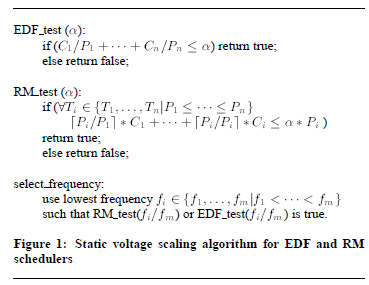
\includegraphics{./images/fig01.png}
	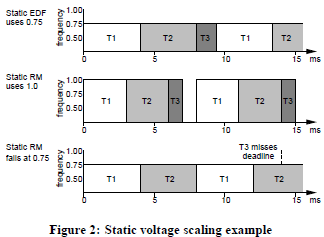
\includegraphics{./images/fig02.png}
\end{figure}
\begin{figure}[h!]
	\centering
	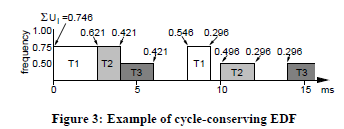
\includegraphics{./images/fig03.png}
	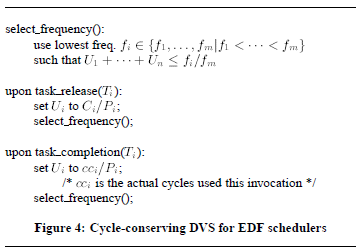
\includegraphics{./images/fig04.png}
\end{figure}
\begin{figure}[h!]
	\centering
	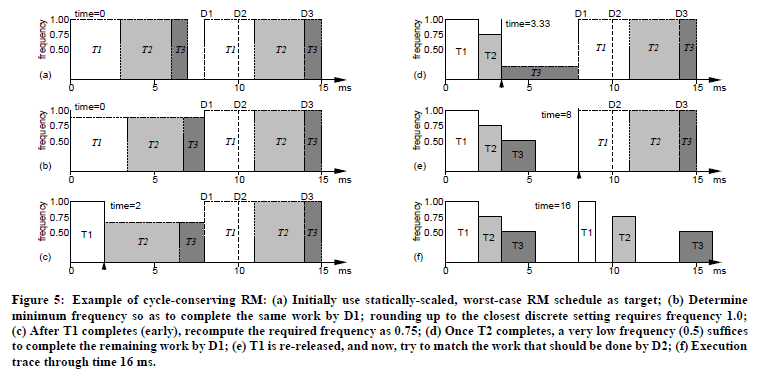
\includegraphics{./images/fig05.png}
	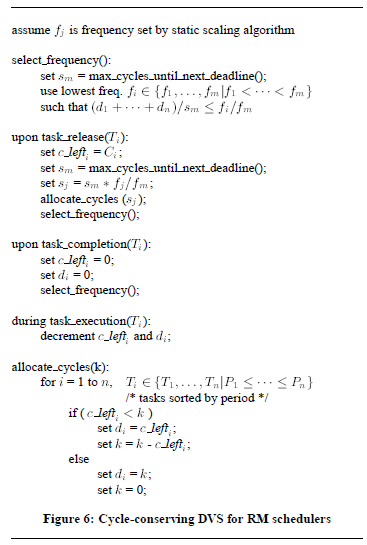
\includegraphics{./images/fig06.png}
\end{figure}
\begin{figure}[h!]
	\centering
	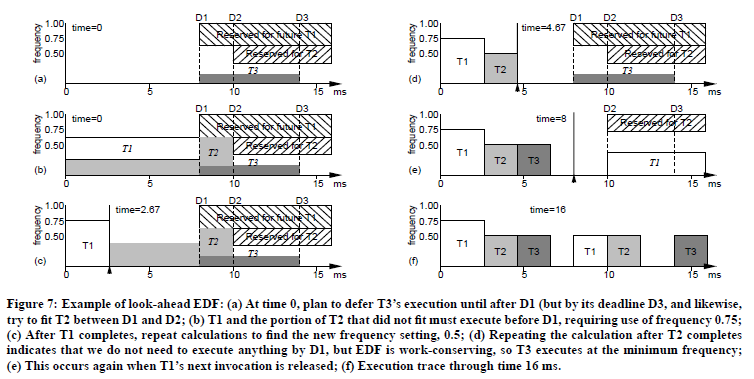
\includegraphics{./images/fig07.png}
	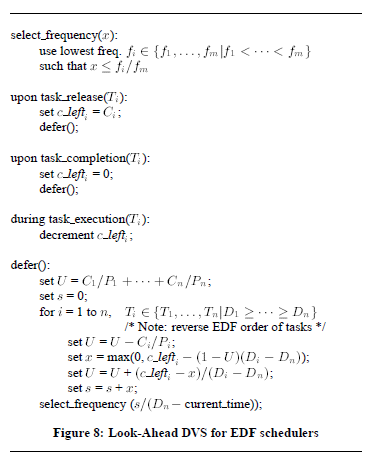
\includegraphics{./images/fig08.png}
\end{figure}
\begin{figure}[h!]
	\centering
	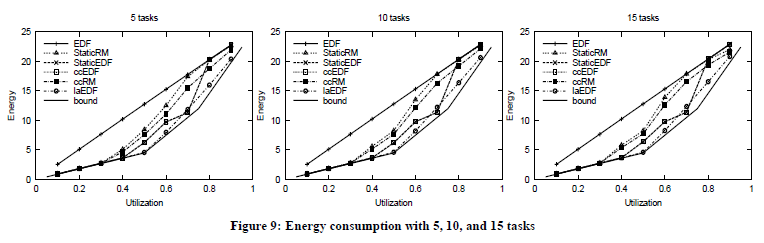
\includegraphics{./images/fig09.png}
	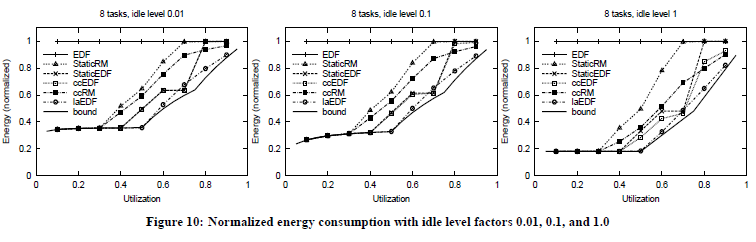
\includegraphics{./images/fig10.png}	
\end{figure}
\begin{figure}[h!]
	\centering
	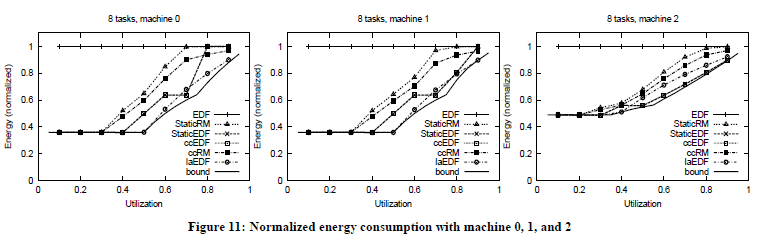
\includegraphics{./images/fig11.png}
	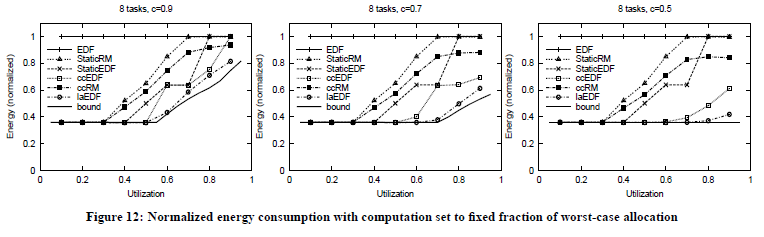
\includegraphics{./images/fig12.png}
\end{figure}
\begin{figure}[h!]
	\centering
	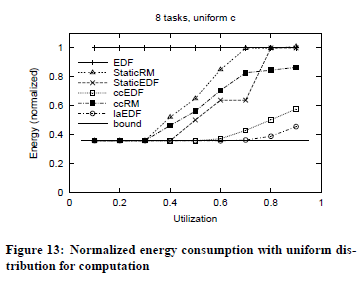
\includegraphics{./images/fig13.png}
	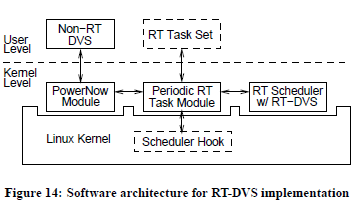
\includegraphics{./images/fig14.png}
\end{figure}
\begin{figure}[h!]
	\centering
	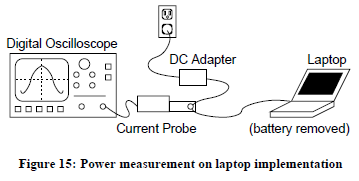
\includegraphics{./images/fig15.png}
	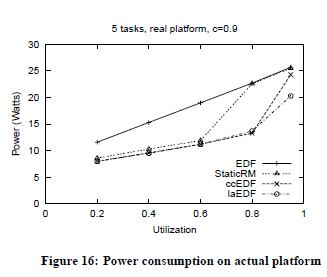
\includegraphics{./images/fig16.png}
\end{figure}
\begin{figure}[h!]
	\centering
	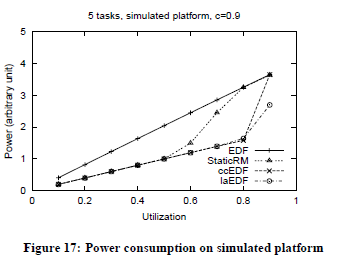
\includegraphics{./images/fig17.png}
\end{figure}

\begin{figure}[h!]
	\centering
	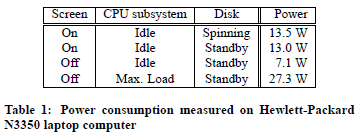
\includegraphics{./images/table1.png}
	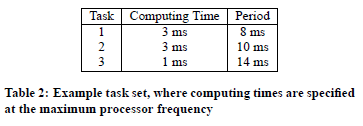
\includegraphics{./images/table2.png}
\end{figure}

\begin{figure}[h!]
	\centering
	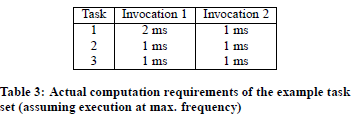
\includegraphics{./images/table3.png}
	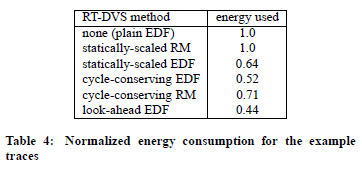
\includegraphics{./images/table4.png}
\end{figure}
\end{document}

